\section{Wikipedia}
\label{sec:wikipedia}

I'm not going to introduce what is \href{http://www.wikipedia.org/}{Wikipedia}, you know what Wikipedia is. I will write about what is not and how Wikipedia community is governed by rules using tools for this mean.

\par Everything revolves around \textit{"citation needed"}quotation.
\\\href{http://gsyc.urjc.es/~mvidal/}{Miguel Vidal} explains the Wikipedia community during the talk through the vision of a Wikipedian. A quick look at what is not Wikipedia

\begin{itemize}
	\item Is not a dictionary.
	\item Is not a blog.
	\item Is not a centralized image bucket.
	\item Is not a web of links.
	\item Is not a collection of meaningless information.
\end{itemize} Wikipedia is a Free Encyclopedia \textit{(yes,I failed, I finally described the meaning of wikipedia :))}with \href{http://creativecommons.org/licenses/by-sa/3.0/}{Creative Commons By Share Alike} (CC-BY-SA) License.

\subsection{Technologies}

\par Wikipedia, Wikipedia, Wikis everywhere ! What was before ? Wiki or Wikipedia ? Wiki was created in march of 1995 by\href{http://c2.com/~ward/}{Ward Cunningham} expert software developer, pattern designer and extreme programing pionner. He defined Wiki as \textit{"The simplest online database that could possibly work"}.

\par Wiki is a content management system focused in team collaboration development. Easy collaboration and visualization for a wiki gives disseminated widely results among developers. The key point is the change history associated with each of the pages. The tool allows you to navigate through the story and find out who did what and when. The more information is saved, the more will learn. Then in 2001 he received a big boost from wikipedia to be chosen as the basis for creating the free encyclopedia that during the 2000s was on everyone's lips (anyone who knew the wikipedia), developers, architects, lawyers, children, teachers, etc..

\par The use of wikis is widespread in software development projects as it allows the integration of collaborative document usage. It uses a simple markup language to represent the text in an agile as a html.

\par The Wiki used in Wikipedia is \textit{\href{http://www.mediawiki.org/wiki/MediaWiki}{MediaWiki}} licensed under the \href{http://www.gnu.org/licenses/gpl.html}{GNU GPLv3}. It was developed specifically for the project by \href{http://magnusmanske.de/}{Magnus Manske}. Today has many users who create their Wikis with MediaWiki software.

\par Although the only lack of wikis, is \textit{markup languages​​ unification} and therefore the need for \textit{WYSIWYG} (\textbf{w}hat \textbf{y}ou \textbf{s}ee \textbf{i}s \textbf{w}hat \textbf{y}ou \textbf{g}et) editors for each type of language. At the end, allows to choose one that best suits for each needs.

\subsection{How to Contribute}

\par In Wikipedia contribute is easier that it seems. Go to a Wiki ie \href{http://en.wikipedia.org/wiki/Software_release_life_cycle}{Software release life cycle} and click \textit{edit} button, add your content and save. That's all, no registrations, no forms, no personal data, edit and save.

\begin{figure}[H]
    \centering
    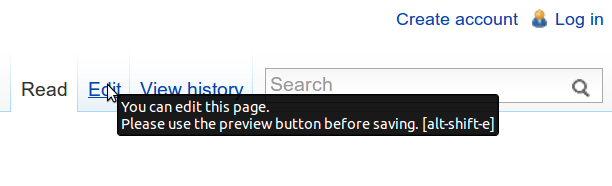
\includegraphics[width=\textwidth]{wiki-edit-button}
    \caption{Wikipedia edit button}
    \label{wiki-edit}
\end{figure}

\par This is your first\textit{affaire}with Wikipedia could be the last only if you want.

Wikipedia has a dedicated domain to Community in \href{http://en.wikipedia.org/wiki/Wikipedia:Community_portal}{Community Portal}:
\begin{quote}
    \textit{"The Community portal is a place to find collaborations, tasks, and news about English Wikipedia."}
\end{quote}

\par There is a guide to start to contribute to Wikipedia throught different ways.

\par \textbf{Important:}Wikipedia is divided in sub communities per each language, this sample is from English Wikipedia.

\begin{itemize}
	\item \textit{Help desk} guides users to learn how to edit using Wiki syntax. How to create an article, describe references, links, citations, relate articles, how to write a Wiki.
	\item In \textit{Reference desk}; you can ask questions to librarians to guide you through Wikipedia inside articles.
	\item \textit{Peer editing} help is a menthoring program for newbies in Wikipedia called TeaHouse. Very interesting part in Community to guide users not only with described rules in more Wikis, community users help to others to interact and use Wikipedia hand by hand with a menthor from Wikipedia. Human communication at least. Very important and appreciated.
	\item \textit{Village pump} is a discussion forum for Wikipedia technical issues, policies, proposals, new ideas. Community discuss policies for Wikipedia reasoning to increase Freedoms in Free Encyclopedia Open Community.
	\item \textit{Dispute resolution}, always are disputes, complains, differences between contributors. This guide tries to resolve them before they exists explaining rules of respect inside Wikipedia and in case you get in the middle of a flame discussion how you can handle this problem and try not to become personal. Always guide yourself from your reasonings.
\end{itemize} I hope you enjoyed and discovered new sections in Wikipedia because is not just an Encyclopedia (Free Encyclopedia :)), is a big community helping each other sharing knowledge with everyone. \textit{People helping people.}

% section wikipedia (end)